\chapter{Pilotforsøg}\vspace{-.75cm}
\textit{Dette bilag beskriver pilotforsøget, som undersøger en række essentielle faktorer i forhold til problemløsningens aspekter.}

\section{Teori}
\textbf{Grundlæggende teori eller henvis tilbage bevægelsesanalysen (Hvis der er en)}

\section{Formål}
Formålet for pilotforsøget er at undersøge en række essentielle faktorer i forbindelse med gang, løb og cykling. De resultater som pilotforsøget medfører, skal benyttes til at konfigurere og tilpasse softwaren for CY8CKIT-043 PSoC 4 M-Series Prototyping Kit, således denne kan opfylde kravene beskrevet i \secref{succeskrav}. \newline
Det sluttelige system skal dermed kunne registrere de enkelte aktiviter, samt adskille aktiviteterne automatisk. Til dette formål har det teoretiske afsnit, \secref{TEORI OM SENSOR}, vist, at et accelerometer og et gyroskop vil være fordelagtigt at benytte. I forlængelse af dette, undersøges det hvorvidt placeringen af sensorerne har en betydning for signalets udformning. Ydermere skal signalets frekvensområde bestemmes. \newline
Formålet med pilotforsøget er dermed:
\begin{itemize}
\item At undersøge signalernes udformning fra accelerometer og gyroskop ved aktiviteterne; gang, løb og cykling. 
\item At undersøge 3 forudbestemte placeringer på underbenets betydning for signalernes udformning.
\item At bestemme frekvensområdet for signalerne.
\end{itemize}

%er det nødvendigt at kende signalets frekvensindhold og vide, hvordan forskellige aktivitetsformer påvirker systemet. Målingerne skal undersøges for at kunne lave en algoritme, som kan få sensoren til at skelne imellem de pågældende aktivitetsformer. Derudover skal det bestemmes, hvor sensoren skal placeres på kroppen for mest optimalt udbytte. Derfor er formålet med pilotforsøget følgende:
%\begin{itemize}
%	\item Bestemme hvordan sensoren påvirkes af gang, løb og cykling. (Undersøge signalets udformning for accelerometer og gyroskop ved aktiviteterne; løb, gang og cykling. 
%		- Ligeledes at undersøge placeringen af sensoren ift. påvirkning af signalet.	
%	\item Undersøge hvor mange g-kræfter sensorens målinger ændrer sig alt efter placering på kroppen.
%	\item Undersøge bevægelsesmønstret i signalet i forhold til placering af sensor.
%	\item Bestemme frekvensindholdet for signalet.
%\end{itemize}

\section{Metode}
Forsøgets metode er bestemt og udført med hensyn til at opfylde de formål som er opstillet som pilotforsøgets formål. \newline
Forsøgets metode involverer henholdsvis de materialer der skal benyttes samt den fremgangsmåde som ligger til grund for udførelsen.

\subsection{Materialer}
\begin{itemize}
	\item Løbebånd med justerbar hastighed og sikkerhedsbæresele.
	\item Motionscykel.
	\item Shimmer3 sensor med tilhørende holder og strap.
	\item (Sports)tape
	\item Computer med følgende software:
	\begin{itemize}
		\item Labview.
		\item Shimmer sensing.
	\end{itemize}
\end{itemize}

\subsection{Fremgangsmåde}
Inden forsøget skal computeren med programmet Multi Shimmer Sync forbindes via Bluetooth med Shimmer3 sensoren. Herefter kalibreres Shimmer3 accelerometeret ved hjælp af kalibreringsklodsen og samplingsfrekvensen indstilles til 500 Hz.\fxnote{Gyroskop trækker for meget, og systemet vil selv sige til, hvis frekvensen er for høj - sættes typisk til 1024 Hz, men derfor sættes den i dette tilfælde kun til 500 Hz}\fxnote{Skal det her slettes?} %Alle andre har indstillet til 1024 Hz, men kan ikke sige hvorfor.
%Der oprettes en mappe for hver forsøgsperson, som yderligere inddeles i fire mapper efter aktivitetsform. Herunder navngives datafilerne fra målingerne i forhold til placering af sensor, som for eksempel "Forsoegsperson\_1 $\rightarrow$ Gang $\rightarrow$ Ankel".\fxnote{Diskuterres om det er for dybdegående - nogle er for og andre er imod} 
Der foretages en testmåling med sensoren, hvor den tændes kortvarigt mens den påvirkes med 1 g. Hvis data fra denne testmåling optages og skildres korrekt er sensoren klar til forsøget.

Forsøget udføres med fire forsøgspersoner. Hver forsøgsperson skal henholdsvis gå, løbe og cykle. Derudover foretages en måling, hvor forsøgspersonen starter fra hvile og med konstant stigningsintervaller skal opnå egen makshastighed. Hvor hver af disse fire målinger skal sensoren placeres på tre forskellige steder, som kan ses på \figref{fig:sensor_placering}.  %Dette giver $4 \cdot 3 = 12$ målinger for hver forsøgsperson og derfor 48 målinger i alt. Derfor er korrekt placering og navngivning af datafilerne yderst essentiel. \\ 
Gang og løb er henholdsvis inddelt i tre hastighedstrin, hvorfor der i pilotforsøget er valgt den midterste af de tre værdier for begge. For gang er dette 3 mph = 4,8 $\sfrac{km}{t}$, og for løb 7mph = 11.3 $\sfrac{km}{t}$. 
%Gang har tre hastigheder - slentre med 2 mph, almindelig gang med 3 mph og frisk gang med 4 mph. Derfor er almindelig gang valgt som tempoet for gangmålingen, hvilket er 3 mph = 4,8 $\sfrac{km}{t}$.\fxnote{Miles per hour omregnes til kilometer i timen ved at gange med 1,61} Løb har ligeledes tre hastigheder - 6, 7 og 8 mph. Derfor er der igen valgt midtværdien på 7mph = 11.3 $\sfrac{km}{t}$ til løbemålingen. 
Cykling kan have en moderat intensitet på 10-12 mph eller en høj intensitet på 12-14 mph. Derfor er midtpunktet ligeledes valgt, som er 12 mph = 19,3 $\sfrac{km}{t}$.\citep{Miles2007} \\
%Inden optagelse af data påbegyndes, skal forsøgspersonen have udført den pågældende aktivitet i et minut for at sikre homogen cyklus i den fysiske udførsel. \\
Sensoren skal placeres tre forskellige steder under hvert forsøg på forsøgspersonens højre ben: proximalt over den laterale malleolus, medialt på den ventrale side af tibia og distalt for patella, som illustreret på \figref{fig:sensor_placering}.
\begin{figure}[H]
	\centering
	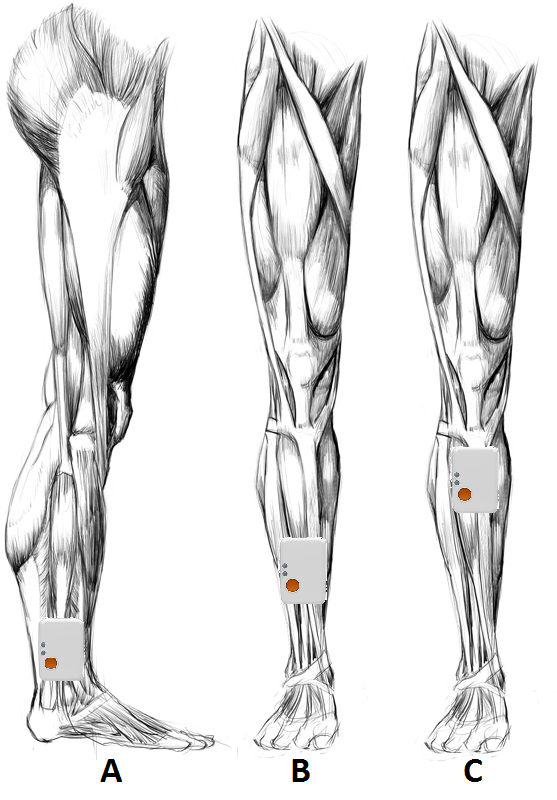
\includegraphics[scale=0.6]{figures/qBilag/Sensor_placering.png}
	\caption{På figuren ses, hvor sensoren skal placeres under pilotforsøget. Placering A viser sensoren siddende proximalt over den laterale malleolus. Placering B illustrerer sensoren, når den er medialt på den ventrale side af tibia. I placering C er sensoren distalt for patella. (Modificeret fra \cite{Perna2016,Shimmer2016})}
	\label{fig:sensor_placering}
\end{figure}
\begin{itemize}
	\item Software punkt...
	\item Kalibrerings punkt....
	\item Forsøgspersonen får fastgjort sensoren i placering A, B eller C - se \figref{fig:sensor_placering}, og gør klar til den pågældende aktivitet ved et stå på kanten af løbebåndet eller sætte sig op på cyklen. Ved aktiviteter på løbebånd skal forsøgspersonen bære sikkerhedsbæresele, som beskytter i tilfælde af fald.
	\begin{itemize}
		\item Ved gang står forsøgspersonen stille på løbebåndet. Optagning af data påbegyndes i 10 sekunder for at optage en baseline for sensorens påvirkning. Herefter træder forsøgspersonen op på løbebåndet og får 20 sekunder til at opnå homogen cyklus i den fysiske udførsel og til, at løbebåndet når op på 4.8 $\sfrac{km}{t}$. Efter disse 20 sekunder optages der yderligere et minut, hvorefter dataoptagelsen stoppes.
		\item Ved løb står forsøgspersonen stille på løbebåndet. Optagning af data påbegyndes i 10 sekunder for at optage en baseline for sensorens påvirkning. Herefter træder forsøgspersonen op på løbebåndet og får 20 sekunder til at opnå homogen cyklus i den fysiske udførsel og til, at løbebåndet når op på 11.3 $\sfrac{km}{t}$. Efter disse 20 sekunder optages der yderligere et minut, hvorefter dataoptagelsen stoppes.
		\item Ved stigning af intensitet skal forsøgspersonen stå stille på løbebåndet mens optagningen påbegyndes og optager en 10 sekunders baseline. Herefter skal løbebåndets hastighed stige fast med et konstant tidsinterval indtil maksspurt er opnået. Dette er en subjektiv vurdering, hvorfor den konstante stigning i hastighed er essentiel og skal noteres i forhold til tid.
		\item Ved cykling skal forsøgspersonen sidde på cyklen og have højre pedal placeret tilnærmelsesvist helt i bund. Der optages en 10 sekunders baseline, hvorefter forsøgspersonen hurtigst muligt og uden at skifte gear skal komme op på 20.9 $\sfrac{km}{t}$. Når dette er opnået, optages signalet i yderligere et minut, hvorefter dataoptagelsen stoppes.
	\end{itemize}
	\item Efter hver måling skal forsøgspersonen restituere i 10 minutter for at sikre, at der ikke sker en kompensering i gang- eller løbecyklus på grund af træthed. %Der tages dog ikke højde for muskeltræthed, da det vurderes, at fysisk aktivitet af denne form ikke vil lede til muskeltræthed inden for disse korte intervaller.\fxnote{Skal vi have en kilde på det her?}
	\item Den pågældende fysiske aktivitet gentages tre gange for hver forsøgsperson, da sensoren skal placeres anderledes for hver gang. Sensoren Shimmer3 skal kalibreres for hvert placeringsskifte og placeringen af sensoren skal markeres på forsøgspersonen. Derved sikres der, at forsøget kan gentages med sammme placering af sensor.
\end{itemize}

\section{Databehandling}

\section{Resultater}

\section{Diskussion}

\section{Konklusion}

%% Opgaver - rettelser
% Man skal markere på forsøgspersonen med tush eller andet hvor sensoren skal placeres